%==============================================================================
%  BCCCE 2027 - PAPER TEMPLATE (LaTeX)
%  5th International Balkans Conference on Challenges of Civil Engineering
%  (BCCCE 2027), 13-15 May 2027, EPOKA University, Tirana, Albania
%
%  Compile with pdfLaTeX. On Overleaf select "pdfLaTeX" (default).
%  This file is fully self-contained: the example figure is drawn with pgfplots,
%  so no external image is required.
%
%  Formatting rules reproduced from the official Word template:
%    - A4 page, 25 mm margins on all sides
%    - Header and footer 15 mm from the paper edge
%    - Times New Roman, 12 pt body, single line spacing, justified
%    - Body paragraphs: 10 mm first-line indent, no blank line between them
%    - Title 14 pt bold; author names 12 pt; affiliations 10 pt italic
%    - Section headings 12 pt bold UPPERCASE; subheadings 12 pt bold
%    - Maximum length 10 pages including figures, tables and references
%    - English (British) and SI units throughout
%
%  NOTE ON FONTS
%    This template uses "mathptmx" (a Times New Roman equivalent) so that it
%    compiles anywhere with pdfLaTeX. To use the genuine Times New Roman font
%    instead, compile with XeLaTeX and replace the mathptmx line below with:
%        \usepackage{fontspec}
%        \setmainfont{Times New Roman}
%==============================================================================
\documentclass[a4paper,12pt]{article}

%------------------------------------------------------------------ fonts -----
\usepackage[T1]{fontenc}
\usepackage[utf8]{inputenc}
\usepackage{mathptmx}          % Times New Roman for text and mathematics

%--------------------------------------------------------------- page layout --
\usepackage[a4paper,
            left=25mm, right=25mm, top=25mm, bottom=25mm,
            headsep=5mm, footskip=10mm]{geometry}
% headsep/footskip chosen so the header and footer sit 15 mm from the edge.

%------------------------------------------------------------- header/footer --
\usepackage{fancyhdr}
\setlength{\headheight}{14pt}
\pagestyle{fancy}
\fancyhf{}
\fancyhead[C]{\fontsize{8}{10}\selectfont\itshape
  5\textsuperscript{th} International Balkans Conference on Challenges of Civil
  Engineering (BCCCE 2027), 13--15 May 2027}
\fancyfoot[C]{\fontsize{10}{12}\selectfont \thepage}
\renewcommand{\headrulewidth}{0pt}
\renewcommand{\footrulewidth}{0pt}

%------------------------------------------------------------- section styles -
\usepackage{titlesec}
% Section: 12 pt bold, UPPERCASE, "1  INTRODUCTION"
\titleformat{\section}
  {\normalfont\fontsize{12}{14}\bfseries\MakeUppercase}
  {\thesection}{1em}{}
% Subsection: 12 pt bold, "2.1  Fonts"
\titleformat{\subsection}
  {\normalfont\fontsize{12}{14}\bfseries}
  {\thesubsection}{1em}{}
% Spacing before/after headings (matches the Word template)
\titlespacing*{\section}{0pt}{12pt}{8pt}
\titlespacing*{\subsection}{0pt}{8pt}{6pt}

%--------------------------------------------------------------- captions -----
\usepackage{caption}
\captionsetup{labelsep=period, font=normalsize, justification=centering,
              singlelinecheck=true}
\captionsetup[table]{position=above}
\captionsetup[figure]{position=below}

%----------------------------------------------------------------- utilities --
\usepackage{graphicx}
\usepackage{amsmath}
\usepackage{booktabs}
\usepackage{array}
\usepackage{float}         % enables [H] so tables/figures stay where written
\usepackage{indentfirst}   % indent the first paragraph after each heading too
\usepackage{pgfplots}      % native example figure (no external image needed)
\pgfplotsset{compat=1.18}

%------------------------------------------------------- body paragraph rules -
\setlength{\parindent}{10mm}   % first-line indent
\setlength{\parskip}{0pt}      % no blank line between paragraphs
\linespread{1.0}               % single line spacing
\sloppy                        % avoids overfull lines in justified text

\begin{document}
%==============================================================================
%  TITLE BLOCK
%==============================================================================
\begin{center}
  {\fontsize{14}{16}\selectfont\bfseries Title of Paper}\par
  \vspace{12pt}
  {\fontsize{12}{14}\selectfont
   Name Surname\textsuperscript{1}, Name Surname\textsuperscript{2}}\par
  \vspace{4pt}
  {\fontsize{10}{12}\selectfont\itshape
   \textsuperscript{1}Department of Civil Engineering, Faculty of Architecture
   and Engineering, EPOKA University, Tirana 1032, Albania\\
   \textsuperscript{2}Department, Faculty, Institution, Address, Country}\par
\end{center}
\vspace{8pt}

%==============================================================================
%  ABSTRACT
%==============================================================================
\section*{Abstract}
This file provides a template for writing papers for the BCCCE Conference. The
proceedings will be published in electronic format. The full paper shall be
written in compliance with these instructions. It will be converted into
Portable Document Format (PDF) before publishing.

An abstract not exceeding 300 words should appear at the top of the first page,
after the title of the paper, in the abstract section.

\vspace{6pt}
\noindent\textbf{Keywords:} keyword one, keyword two, keyword three, keyword four

%==============================================================================
%  1  INTRODUCTION
%==============================================================================
\section{Introduction}
The main text of the manuscript should be divided into sections. The paper
length, including figures, tables and references, should \textbf{not exceed
10 pages}.

Papers are to be prepared in English (British) and SI units shall be used.

%==============================================================================
%  2  PAPER FORMAT
%==============================================================================
\section{Paper Format}
The authors should use this template file to write their manuscripts. Please
note the following details: this template is on A4 page format with 25 mm
margins on the left, right, top and bottom. The header and footer shall be
positioned 15 mm from the edge.

All text paragraphs should be single spaced. Double spacing should only be used
before and after headings and subheadings, as shown in this example. The
position and style of headings and subheadings should follow this example. No
spaces should be placed between paragraphs. Please do not change any of the
above-mentioned page, paragraph and font settings.

\subsection{Fonts}
Papers should use 12-point Times New Roman font. The styles available are
\textbf{bold}, \textit{italic} and \underline{underlined}.

It is recommended that text in figures is not smaller than 10-point font size.

\subsection{Tables and Figures}
Figure captions and table headings should be sufficient to explain the figure
or table without needing to refer to the text. Figures and tables not cited in
the text should not be presented.

The following is the example for Table~\ref{tab:example}.

\begin{table}[H]
  \centering
  \caption{Title of Example Table}
  \label{tab:example}
  \begin{tabular}{lccc}
    \toprule
                        & $\mathbf{U_m}$ & $\mathbf{U_{mak}}$ & $\mathbf{U_m / U_{mak}}$ \\
    \midrule
    \textbf{Example\_1} & 0.600 & 0.950 & 0.632 \\
    \textbf{Example\_2} & 0.529 & 0.881 & 0.600 \\
    \textbf{Example\_3} & 0.565 & 0.932 & 0.607 \\
    \textbf{Example\_4} & 0.518 & 0.865 & 0.599 \\
    \textbf{Example\_5} & 0.536 & 0.885 & 0.605 \\
    \textbf{Example\_6} & 0.516 & 0.885 & 0.583 \\
    \bottomrule
  \end{tabular}
\end{table}

Tables and figures should be placed close after their first reference in the
text. All figures and tables should be numbered with Arabic numerals. Table
headings should be centred above the tables. Figure captions should be centred
below the figures. An example is shown in Figure~\ref{fig:example}.

\begin{figure}[H]
  \centering
  % To use your own image instead, delete the tikzpicture below and uncomment:
  % \includegraphics[width=0.6\linewidth]{your_figure.png}
  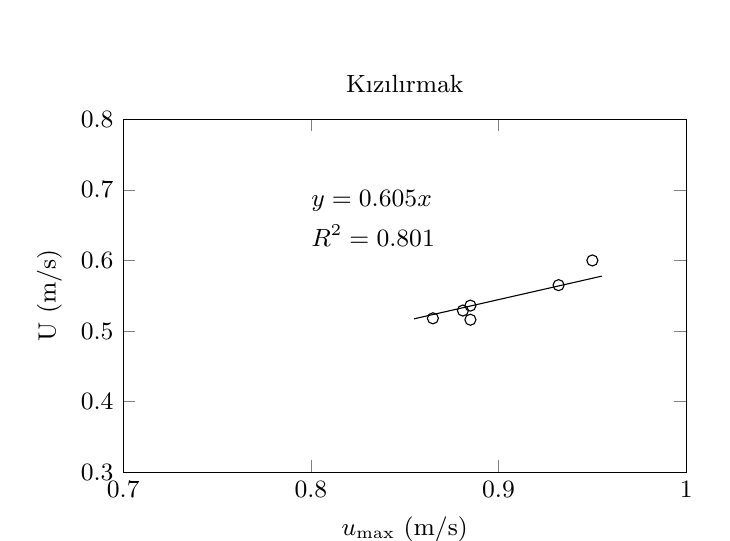
\begin{tikzpicture}
    \begin{axis}[
        width=0.72\linewidth, height=0.50\linewidth,
        title={K{\i}z{\i}l{\i}rmak},
        xlabel={$u_{\max}$ (m/s)}, ylabel={U (m/s)},
        xmin=0.7, xmax=1.0, ymin=0.3, ymax=0.8,
        xtick={0.7,0.8,0.9,1.0},
        ytick={0.3,0.4,0.5,0.6,0.7,0.8},
        title style={font=\small}, label style={font=\small},
        tick label style={font=\small},
      ]
      % Data points (u_max, U), taken from Table 1
      \addplot[only marks, mark=o, mark size=2pt, black] coordinates {
        (0.950,0.600) (0.881,0.529) (0.932,0.565)
        (0.865,0.518) (0.885,0.536) (0.885,0.516)
      };
      % Linear trend through the origin: y = 0.605 x
      \addplot[no marks, black, domain=0.855:0.955, samples=2] {0.605*x};
      \node[anchor=west, font=\small] at (axis cs:0.795,0.685) {$y = 0.605x$};
      \node[anchor=west, font=\small] at (axis cs:0.795,0.635) {$R^{2} = 0.801$};
    \end{axis}
  \end{tikzpicture}
  \caption{Relation between U and $u_{\max}$ for K{\i}z{\i}l{\i}rmak station}
  \label{fig:example}
\end{figure}

\subsection{Equations}
Each equation should be presented on a separate line from the text, with a
blank space above and below. Equations should be clear, and expressions used
should be explained in the text. The equations should be numbered consecutively
at the outer right margin, as shown in Eq.~(\ref{eq:1}) and~(\ref{eq:2}) below:

\begin{equation}
  Q = VA
  \label{eq:1}
\end{equation}

\begin{equation}
  \varepsilon(\%) = \left| \frac{Q - Q_{M}}{Q} \right| \times 100
  \label{eq:2}
\end{equation}

%==============================================================================
%  3  CONCLUSION
%==============================================================================
\section{Conclusion}
This section should state the most important conclusions of the paper.

%==============================================================================
%  REFERENCES
%   Cite in the text with square brackets, e.g. [1-3].
%==============================================================================
\begin{thebibliography}{99}
\setlength{\itemsep}{2pt}

\bibitem{ref1}
Araujo, J.C. and Chaudhry, F.H. (1996) Experimental evaluation of 2-D entropy
model for open channel flow. \textit{Journal of Hydraulic Engineering, ASCE},
\textbf{124}(10), 1064--1067.

\bibitem{ref2}
Chow, V.T. (1959) Open Channel Hydraulics. \textit{McGraw-Hill Book Co.}, New
York, NY, USA.

\bibitem{ref3}
Ard{\i}\c{c}l{\i}o\u{g}lu, M., Gen\c{c}, O., Girayhan, A. and K{\i}rkg\"{o}z,
M.S. (2008) ADV measurements of velocity distributions in natural rivers.
\textit{International Conference on Fluvial Hydraulics}, \c{C}e\c{s}me, {\.I}zmir.

\end{thebibliography}

\end{document}